% Drawing 81/01-1 -- folder 81, batch 01, archive page 9 (PDF page 10).
% Transcription: feuillet de dessins, sans texte. Trois rangées de disques coupés par des cordes (droites ou arcs), parfois concourantes en un point marqué, une région parfois hachurée ; sous chaque disque ou groupe de disques réuni par une accolade, un petit graphe : un point, deux points, un segment, trois points, un segment et un point, un chemin à trois sommets, un triangle — apparemment le graphe dont les sommets sont les cordes et les arêtes leurs croisements. Plusieurs dessins sont marqués « ok » de sa main (le disque à trois cordes concourantes au-dessus d'un segment, le disque au triangle hachuré au-dessus du triangle, avec en variante « ou » un disque à cordes concourantes) ; sous une rangée de disques à quatre cordes parallèles, un « ? ». En bas à droite, des lignes brisées épaisses
% Kind: page of disks cut by chords, with their crossing graphs. Method 2 (schematic redraw from the facsimile). Status: ok.
% Notes: Redrawn disk by disk from a fresh crop of p. 9 (issue 128), 1 unit = 1.8 mm. Each disk is an ellipse fitted to his outline; every straight chord is clipped to that ellipse, so that it ends exactly on it, and where a disk carries a marked point the chords are drawn through that one point; the short curved chords (caps) are drawn as curves whose ends lie on the outline; heavy segments are drawn between the computed crossings of their chords (the X of the 7th disk of row 1, the two disks with a heavy middle bar and the ok disk of row 3), and the hatched triangle of row 1 between the crossings of its three chords. Row 1: one chord, two chords, X through a point (ok), three parallel chords and the disk with three caps (joined by a brace, three points ringed), the disk with a point and a cap (segment and point ringed), the X with a heavy bar and a third chord (ok, path of three vertices), the hatched triangle (ok, triangle), and "(ou" a disk with three chords through a point. Row 2: four parallel chords (outer two curved), three chords and a small cap, four caps (brace, four points, "?"); four disks with two chords through a point and caps, the last with a stroke rising from it (brace; segment and two points). Row 3: two pairs of chords through two points (ok; two segments); a disk with three chords, a curved fourth and a hatched region, and two disks with two chords and a heavy cross bar (brace; path of three vertices and a point); the ok disk with four chords and its heavy path (path of four vertices); the thick broken line at the bottom right and the strokes near it (a heavy stroke from the last graph, faint pencil strokes). Left out: small ticks where he starts an outline or a chord, an ink blot in the last disk of row 2 and a smudge under the ou-variant. Still differs: the outlines are ellipses (some of his are rounder at a corner); the hatched region of the first disk of row 3 is a reading of loose zigzag strokes (it could also be a scribbling-out). Redrawn 2026-11-09 (issue 128): to check again. Revised 2026-11-09 after Michel's check (#136): yes, as redrawn; the region of the second disk of row 3 is hatched (a hatched polygon bounded by the three chords and the curved fourth side), not scribbled out; ok.
% Coordinates: 1 unit = 1.8 mm = 1/100 of the crop width (bbox in page fractions: [0.1, 0.07, 0.99, 0.51]).
% Redrawn by Claude (claude-opus-5-5), issue #73, 2026-11-09; not checked by a human; not compiled (no TeX in the session).
% Rights: reproduces part of the work -- behind RENDER_TRANSCRIPTS, never published by itself.
\documentclass[tikz,border=3pt]{standalone}
\usepackage{amsmath,amssymb}
\usetikzlibrary{patterns,arrows.meta}
\tikzset{pencil/.style={black!45}, struck/.style={black!35}, mark/.style={circle,draw,inner sep=1.3pt}, pt/.style={circle,fill,inner sep=0.9pt}, opt/.style={circle,draw,fill=white,inner sep=1.1pt}}
\begin{document}
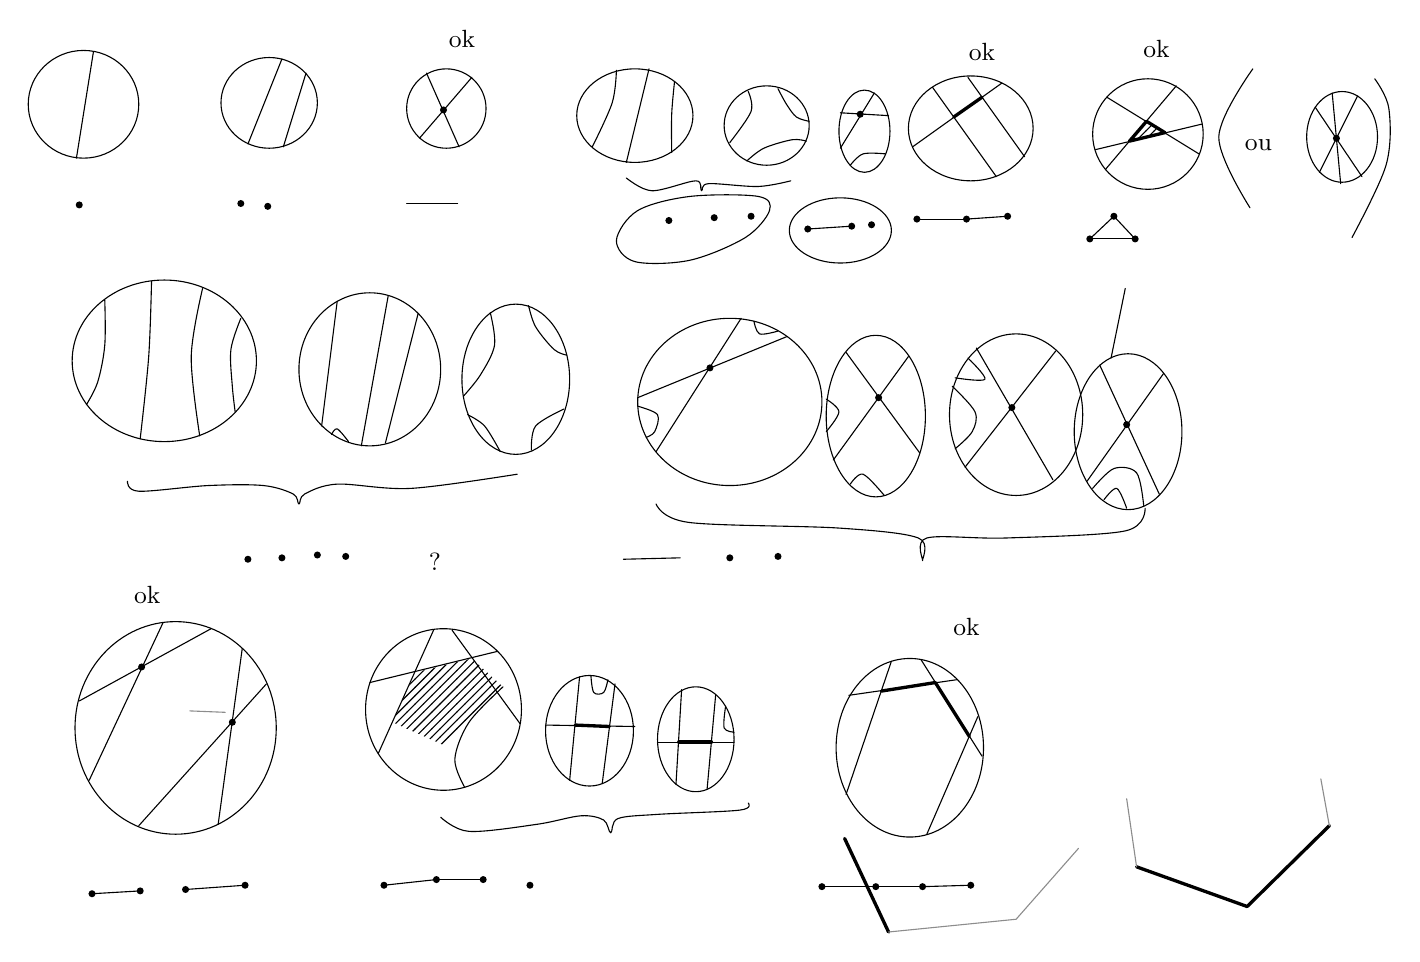
\begin{tikzpicture}[x=1.8mm,y=1.8mm,line cap=round,line join=round,font=\scriptsize]
\draw (6.9,-6.7) ellipse[x radius=3.9, y radius=3.8];
\draw (7.6,-3) -- (6.4,-10.5);
\node[pt] at (6.6,-13.8) {};
\draw (20,-6.6) ellipse[x radius=3.4, y radius=3.2];
\draw (20.9,-3.5) -- (18.5,-9.5);
\draw (22.6,-4.5) -- (21,-9.7);
\node[pt] at (18,-13.7) {};
\node[pt] at (19.9,-13.9) {};
\draw (32.5,-7) ellipse[x radius=2.8, y radius=2.8];
\node[pt] at (32.3,-7.1) {};
\draw (33.4,-9.7) -- (31.1,-4.5);
\draw (30.6,-9.1) -- (34.3,-4.8);
\draw (29.7,-13.7) -- (33.3,-13.7);
\node[inner sep=1pt] at (33.6,-2.1) {\small ok};
\draw (45.8,-7.5) ellipse[x radius=4.1, y radius=3.3];
\draw plot[smooth, tension=0.55] coordinates {(44.5,-4.3) (44.2,-6.6) (42.8,-9.7)};
\draw (46.8,-4.2) -- (45.2,-10.8);
\draw plot[smooth, tension=0.55] coordinates {(48.6,-5.1) (48.4,-7.4) (48.4,-10.1)};
\draw (55.1,-8.2) ellipse[x radius=3, y radius=2.8];
\draw plot[smooth, tension=0.55] coordinates {(53.8,-5.8) (54,-7.2) (52.5,-9.4)};
\draw plot[smooth, tension=0.55] coordinates {(55.9,-5.6) (56.5,-6.7) (57.2,-7.6) (58.1,-7.9)};
\draw plot[smooth, tension=0.55] coordinates {(53.7,-10.7) (54.9,-9.8) (56.9,-9.2) (57.9,-9.3)};
\draw plot[smooth, tension=0.55] coordinates {(45.2,-11.9) (47,-12.8) (50.1,-12.1) (50.5,-12.8) (51,-12.3) (54.5,-12.5) (56.8,-12.1)};
\draw plot[smooth cycle, tension=0.55] coordinates {(44.5,-16.3) (46,-14.2) (49.7,-13.2) (54.5,-13.2) (55.3,-14.2) (53.6,-16.1) (49.7,-17.7) (45.8,-17.8)};
\node[pt] at (48.2,-14.9) {};
\node[pt] at (51.4,-14.7) {};
\node[pt] at (54,-14.6) {};
\draw (62,-8.6) ellipse[x radius=1.8, y radius=2.9];
\node[pt] at (61.7,-7.4) {};
\draw (60.3,-7.3) -- (63.7,-7.5);
\draw (62.7,-5.9) -- (60.3,-9.8);
\draw plot[smooth, tension=0.55] coordinates {(61,-11) (61.9,-10.2) (63.5,-10.2)};
\draw (60.3,-15.6) ellipse[x radius=3.6, y radius=2.3];
\draw (58,-15.5) -- (61.1,-15.3);
\node[pt] at (58,-15.5) {};
\node[pt] at (61.1,-15.3) {};
\node[pt] at (62.5,-15.2) {};
\draw (69.5,-8.4) ellipse[x radius=4.4, y radius=3.7];
\draw (66.8,-5.5) -- (71.3,-11.8);
\draw (65.4,-9.7) -- (71.7,-5.2);
\draw (69.3,-4.8) -- (73.3,-10.4);
\draw[very thick] (68.3,-7.6) -- (70.3,-6.2);
\node[inner sep=1pt] at (70.3,-3) {\small ok};
\draw (65.7,-14.8) -- (69.2,-14.8);
\draw (69.2,-14.8) -- (72.1,-14.6);
\node[pt] at (65.7,-14.8) {};
\node[pt] at (69.2,-14.8) {};
\node[pt] at (72.1,-14.6) {};
\draw (82,-8.8) ellipse[x radius=3.9, y radius=3.9];
\draw (84,-5.4) -- (79,-11.3);
\draw (79.1,-6.2) -- (85.6,-10.2);
\draw (78.3,-9.9) -- (85.8,-8.1);
\fill[pattern=north east lines] (81.9,-7.9) -- (83.2,-8.7) -- (80.7,-9.3) -- cycle;
\draw[very thick] (81.9,-7.9) -- (83.2,-8.7) -- (80.7,-9.3) -- cycle;
\node[inner sep=1pt] at (82.6,-2.8) {\small ok};
\draw (79.6,-14.6) -- (77.9,-16.2);
\draw (77.9,-16.2) -- (81.1,-16.2);
\draw (81.1,-16.2) -- (79.6,-14.6);
\node[pt] at (79.6,-14.6) {};
\node[pt] at (77.9,-16.2) {};
\node[pt] at (81.1,-16.2) {};
\draw plot[smooth, tension=0.55] coordinates {(89.4,-4.2) (87,-9) (89.2,-14)};
\node[inner sep=1pt] at (89.8,-9.6) {\small ou};
\draw plot[smooth, tension=0.55] coordinates {(98,-4.9) (99,-7) (98.8,-11) (96.4,-16.1)};
\draw (95.7,-9) ellipse[x radius=2.5, y radius=3.2];
\node[pt] at (95.3,-9.1) {};
\draw (95.6,-12.3) -- (95,-5.9);
\draw (94.1,-11.5) -- (96.8,-6.1);
\draw (97.1,-11.8) -- (93.8,-6.9);
\draw (12.6,-24.8) ellipse[x radius=6.5, y radius=5.7];
\draw plot[smooth, tension=0.55] coordinates {(8.4,-20.5) (8.4,-23.7) (7.9,-26.3) (7.1,-27.9)};
\draw plot[smooth, tension=0.55] coordinates {(11.7,-19.2) (11.5,-24.5) (10.9,-30.3)};
\draw plot[smooth, tension=0.55] coordinates {(15.3,-19.7) (14.5,-24.5) (15.1,-30.1)};
\draw plot[smooth, tension=0.55] coordinates {(18,-21.8) (17.3,-24) (17.4,-26.6) (17.6,-28.4)};
\draw (27.1,-25.4) ellipse[x radius=5, y radius=5.4];
\draw (24.8,-20.6) -- (23.7,-29.4);
\draw (28.4,-20.2) -- (26.5,-30.8);
\draw (30.5,-21.5) -- (28.2,-30.6);
\draw plot[smooth, tension=0.55] coordinates {(24.4,-30) (24.8,-29.6) (25.6,-30.5)};
\draw (37.4,-26.1) ellipse[x radius=3.8, y radius=5.3];
\draw plot[smooth, tension=0.55] coordinates {(35.6,-21.4) (35.9,-23.7) (34.9,-25.8) (33.7,-27.3)};
\draw plot[smooth, tension=0.55] coordinates {(38.3,-20.9) (38.8,-22.4) (40.1,-24) (41,-24.4)};
\draw plot[smooth, tension=0.55] coordinates {(34,-28.6) (35.2,-29.4) (36.3,-31.2)};
\draw plot[smooth, tension=0.55] coordinates {(38.5,-31.1) (38.8,-29.4) (40.8,-28.2)};
\draw plot[smooth, tension=0.55] coordinates {(10,-33.3) (10.8,-34) (15.7,-33.6) (19.6,-33.6) (21.7,-34.2) (22.1,-34.9) (22.5,-34.2) (24.8,-33.5) (30,-33.8) (37.5,-32.8)};
\node[pt] at (18.5,-38.8) {};
\node[pt] at (20.9,-38.7) {};
\node[pt] at (23.4,-38.5) {};
\node[pt] at (25.4,-38.6) {};
\node[inner sep=1pt] at (31.7,-39) {\small ?};
\draw (52.5,-27.7) ellipse[x radius=6.5, y radius=5.9];
\node[pt] at (51.1,-25.3) {};
\draw (47.3,-31.2) -- (53.3,-21.8);
\draw (46,-27.4) -- (56.5,-23.1);
\draw plot[smooth, tension=0.55] coordinates {(54.2,-22) (54.6,-22.9) (55.9,-22.7)};
\draw plot[smooth, tension=0.55] coordinates {(46,-28) (47.4,-28.6) (47.2,-29.8) (46.6,-30.2)};
\draw (62.8,-28.7) ellipse[x radius=3.5, y radius=5.7];
\node[pt] at (63,-27.4) {};
\draw (65.9,-31.3) -- (60.7,-24.2);
\draw (59.8,-31.8) -- (65.1,-24.5);
\draw plot[smooth, tension=0.55] coordinates {(59.3,-27.5) (60.2,-28.4) (59.3,-29.8)};
\draw plot[smooth, tension=0.55] coordinates {(61,-33.5) (61.9,-32.8) (63.4,-34.3)};
\draw (72.7,-28.6) ellipse[x radius=4.7, y radius=5.7];
\node[pt] at (72.4,-28.1) {};
\draw (75.3,-33.2) -- (69.9,-23.9);
\draw (69.1,-32.3) -- (75.5,-24.1);
\draw plot[smooth, tension=0.55] coordinates {(68.2,-26.6) (69.8,-28.4) (69.6,-29.8) (68.4,-31)};
\draw plot[smooth, tension=0.55] coordinates {(69.3,-24.6) (70.5,-26.1) (68.4,-26)};
\draw (80.6,-29.8) ellipse[x radius=3.8, y radius=5.5];
\node[pt] at (80.5,-29.3) {};
\draw (82.8,-34.2) -- (78.6,-25.1);
\draw (77.7,-33.3) -- (83.1,-25.7);
\draw plot[smooth, tension=0.55] coordinates {(78.1,-33.8) (79.6,-32.4) (81.2,-32.7) (81.7,-35)};
\draw plot[smooth, tension=0.55] coordinates {(78.9,-34.6) (79.8,-33.8) (80.5,-35.2)};
\draw (80.4,-19.7) -- (79.4,-24.6);
\draw plot[smooth, tension=0.55] coordinates {(47.3,-34.9) (49.6,-36.2) (60.2,-36.6) (65.8,-37.3) (66.1,-38.9) (66.4,-37.3) (72,-37.3) (80.4,-36.8) (81.8,-35.2)};
\draw (45,-38.8) -- (49,-38.7);
\node[pt] at (52.5,-38.7) {};
\node[pt] at (55.9,-38.6) {};
\draw (13.4,-50.7) ellipse[x radius=7.1, y radius=7.5];
\node[pt] at (11,-46.4) {};
\node[pt] at (17.4,-50.3) {};
\draw (7.3,-54.4) -- (12.5,-43.3);
\draw (6.6,-48.8) -- (15.9,-43.7);
\draw (16.4,-57.5) -- (18.1,-45.1);
\draw (10.8,-57.6) -- (19.8,-47.6);
\draw[pencil] (14.4,-49.5) -- (16.9,-49.6);
\node[inner sep=1pt] at (11.4,-41.3) {\small ok};
\draw (7.5,-62.4) -- (10.9,-62.2);
\draw (14.1,-62.1) -- (18.3,-61.8);
\node[pt] at (7.5,-62.4) {};
\node[pt] at (10.9,-62.2) {};
\node[pt] at (14.1,-62.1) {};
\node[pt] at (18.3,-61.8) {};
\draw (32.3,-49.4) ellipse[x radius=5.5, y radius=5.7];
\draw (32.9,-43.8) -- (37.7,-50.4);
\draw (27.1,-47.5) -- (36.1,-45.3);
\draw (27.7,-52.5) -- (31.6,-43.8);
\draw plot[smooth, tension=0.55] coordinates {(36.5,-47.8) (34.1,-50.3) (33.1,-52.9) (33.8,-54.9)};
\fill[pattern=north east lines] (30.3,-46.8) -- (34.3,-45.8) -- (36.5,-47.8) -- (34.1,-50.3) -- (32.5,-52) -- (28.7,-50.3) -- cycle;
\draw (42.6,-50.9) ellipse[x radius=3.1, y radius=3.9];
\draw (41.9,-47.1) -- (41.2,-54.4);
\draw (44.4,-47.6) -- (43.5,-54.6);
\draw (39.5,-50.5) -- (45.8,-50.6);
\draw[very thick] (41.6,-50.5) -- (44,-50.6);
\draw plot[smooth, tension=0.55] coordinates {(42.7,-47) (42.9,-48.2) (43.6,-48.2) (43.9,-47.3)};
\draw (50.1,-51.5) ellipse[x radius=2.7, y radius=3.7];
\draw (49.1,-48) -- (48.7,-54.7);
\draw (51.5,-48.4) -- (50.9,-55);
\draw (47.4,-51.7) -- (52.8,-51.7);
\draw[very thick] (48.9,-51.7) -- (51.2,-51.7);
\draw plot[smooth, tension=0.55] coordinates {(52.2,-49.2) (52.1,-50.7) (52.8,-51)};
\draw plot[smooth, tension=0.55] coordinates {(32.1,-57) (34.1,-58) (38.9,-57.5) (42,-56.9) (43.6,-57.2) (44.1,-58.1) (44.6,-57.1) (47.4,-56.8) (53.2,-56.5) (53.8,-56)};
\draw (28.1,-61.8) -- (31.8,-61.4);
\draw (31.8,-61.4) -- (35.1,-61.4);
\node[pt] at (28.1,-61.8) {};
\node[pt] at (31.8,-61.4) {};
\node[pt] at (35.1,-61.4) {};
\node[pt] at (38.4,-61.8) {};
\draw (65.2,-52.1) ellipse[x radius=5.2, y radius=6.3];
\draw (60.9,-48.4) -- (68.5,-47.3);
\draw (66,-45.9) -- (70.3,-52.7);
\draw (63.9,-46) -- (60.7,-55.4);
\draw (70,-49.9) -- (66.4,-58.2);
\draw[very thick] (63.2,-48.1) -- (67,-47.5);
\draw[very thick] (67,-47.5) -- (69.4,-51.3);
\node[inner sep=1pt] at (69.2,-43.6) {\small ok};
\draw (59,-61.9) -- (62.8,-61.9);
\draw (62.8,-61.9) -- (66.1,-61.9);
\draw (66.1,-61.9) -- (69.5,-61.8);
\node[pt] at (59,-61.9) {};
\node[pt] at (62.8,-61.9) {};
\node[pt] at (66.1,-61.9) {};
\node[pt] at (69.5,-61.8) {};
\draw[very thick] (60.6,-58.5) -- (63.7,-65.1);
\draw[pencil] (63.7,-65.1) -- (72.7,-64.2) -- (77.1,-59.2);
\draw[very thick] (81.2,-60.5) -- (89,-63.3) -- (94.8,-57.6);
\draw[pencil] (80.5,-55.7) -- (81.2,-60.5);
\draw[pencil] (94.8,-57.6) -- (94.2,-54.3);
\end{tikzpicture}
\end{document}
